\section{Logic, Shift and Rotate Instructions}

\begin{concept}{Logic Instructions}\\
Base logic operations (affect only N and Z flags):
\begin{itemize}
  \item \textbf{ANDS}: Bitwise AND (Rdn \& Rm, a \& b)
  \item \textbf{BICS}: Bit Clear (Rdn \& !Rm, a \& ~b)
  \item \textbf{EORS}: Exclusive OR (Rdn \textdollar Rm, a $\wedge$  b)
  \item \textbf{MVNS}: Bitwise NOT (!Rm, ~a)
  \item \textbf{ORRS}: Bitwise OR (Rdn \# Rm, a | b)
\end{itemize}
\end{concept}

\begin{concept}{Shift and Rotate Instructions}\\
Shift operations for binary manipulation:
\begin{itemize}
  \item \textbf{LSLS}: Logical Shift Left ($2^n \cdot Rn$, 0 → LSB)
  \item \textbf{LSRS}: Logical Shift Right ($2^{-n} \cdot Rn$, 0 → MSB)
  \item \textbf{ASRS}: Arithmetic Shift Right ($R^{-n}$, ±MSB → MSB)
  \item \textbf{RORS}: Rotate Right (LSB → MSB)
\end{itemize}

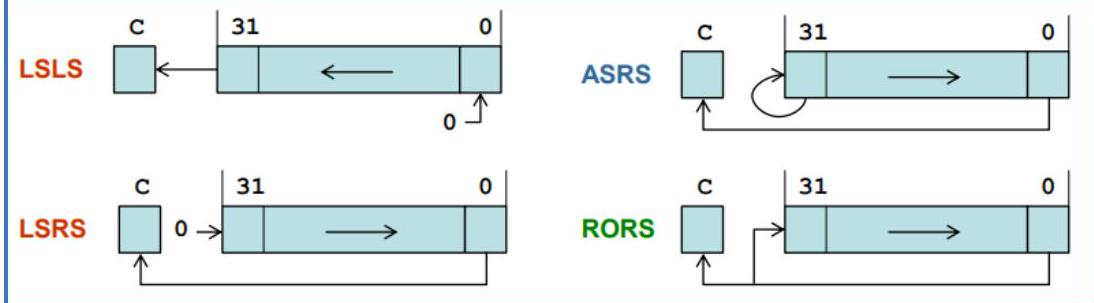
\includegraphics[width=\linewidth]{images/2024_12_29_79e6b22f503fb7b4f718g-06}
\end{concept}

\begin{definition}{Integer Casting}\\
\textbf{Extension (adding bits):}
\begin{itemize}
  \item \textbf{Zero Extension} (unsigned):
    \begin{itemize}
      \item Fill left bits with zero
      \item Example: 1011 → 00001011
    \end{itemize}
  \item \textbf{Sign Extension} (signed):
    \begin{itemize}
      \item Copy sign bit to the left
      \item Example: 1011 → 11111011
    \end{itemize}
\end{itemize}

\textbf{Truncation (removing bits):}
\begin{itemize}
  \item Signed: May change sign
  \item Unsigned: Results in modulo operation
\end{itemize}
\end{definition}

\begin{example2}{Integer Ranges by Word Size}
\textbf{8-bit integers:}
\begin{itemize}
  \item Unsigned: 0 to 255 (0x00 to 0xFF)
  \item Signed: -128 to 127 (0x80 to 0x7F)
\end{itemize}

\textbf{16-bit integers:}
\begin{itemize}
  \item Unsigned: 0 to 65,535 (0x0000 to 0xFFFF)
  \item Signed: -32,768 to 32,767 (0x8000 to 0x7FFF)
\end{itemize}

\textbf{32-bit integers:}
\begin{itemize}
  \item Unsigned: 0 to 4,294,967,295 (0x00000000 to 0xFFFFFFFF)
  \item Signed: -2,147,483,648 to 2,147,483,647 (0x80000000 to 0x7FFFFFFF)
\end{itemize}
\end{example2}

\begin{example2}{Logical Operations}
Common logic operations:
\begin{lstlisting}[language=armasm, style=basesmol]
    ; Logic operations
    ANDS R0, R1         ; R0 = R0 AND R1
    BICS R0, R1         ; R0 = R0 AND NOT R1
    EORS R0, R1         ; R0 = R0 XOR R1
    MVNS R0, R1         ; R0 = NOT R1
    ORRS R0, R1         ; R0 = R0 OR R1
    
    ; Shift operations
    LSLS R0, R1, #2     ; R0 = R1 << 2 (multiply by 4)
    LSRS R0, R1, #1     ; R0 = R1 >> 1 (divide by 2)
    ASRS R0, R1, #2     ; R0 = R1 >> 2 (signed divide by 4)
    RORS R0, R1, #1     ; Rotate R1 right by 1 bit
\end{lstlisting}
\end{example2}

\begin{KR}{Using Logic and Shift Instructions}\\
Steps for bit manipulation:
\begin{enumerate}
  \item Identify required operation (AND, OR, XOR, NOT, shift)
  \item Choose appropriate instruction
  \item Consider effect on flags if relevant
  \item For shifts:
    \begin{itemize}
      \item LSLS for multiplication by $2^n$
      \item LSRS for unsigned division by $2^n$
      \item ASRS for signed division by $2^n$
    \end{itemize}
  \item For logic:
    \begin{itemize}
      \item ANDS for bit masking
      \item ORRS for bit setting
      \item BICS for bit clearing
      \item EORS for bit toggling
    \end{itemize}
\end{enumerate}
\end{KR}